\documentclass[t,pdf]{beamer}
\mode<presentation>{}


\usecolortheme[RGB={196, 30, 58}]{structure}

\usepackage{color}
\usepackage{animate}
\usepackage{tikz}
\usetikzlibrary{shadings,shadows}
\usetikzlibrary{shapes, arrows}
\usetikzlibrary{decorations.pathreplacing,angles,quotes}
\usetikzlibrary{calc}
\usetikzlibrary{positioning}
\usepackage{pgfplots}
\usepackage{graphicx}
\usepackage{adjustbox}
\usepackage{scrextend}
\usepackage{ifthen}

\newcommand{\reference}[1]{{\footnotesize [#1]}}
%\newcommand{\reference}[1]{}

\newboolean{details}
\setboolean{details}{false}


\newcommand{\skipframe}[1]{\ifthenelse{\boolean{details}}{\frame{#1}}{}}

\usepackage{hyperref}
%% Colored hyperlink 
\newcommand{\cref}[2]{\href{#1}{\color{blue}#2}}
%% Colored hyperlink showing link in TT font
% \newcommand{\chref}[1]{\href{#1}{\small\tt \color{blue}#1}}
\newcommand{\hcref}[1]{\cref{#1}{\small\tt #1}}

\usepackage{booktabs,colortbl}

\newcommand{\opos}[1]{#1}
\newcommand{\oneg}[1]{\overline{#1}}
\newcommand{\nil}{\bot}
\newcommand{\lit}{\ell}
%%\newcommand{\implies}{\Rightarrow}
\newcommand{\bitem}{\item[$\bullet$]}

\newcommand{\makenode}[1]{{\mathbf #1}}
\newcommand{\nodeu}{\makenode{u}}
\newcommand{\nodev}{\makenode{v}}
\newcommand{\nodew}{\makenode{w}}
\newcommand{\nodes}{\makenode{s}}
\newcommand{\noder}{\makenode{r}}
\newcommand{\nodep}{\makenode{p}}

\newcommand{\anot}{\oneg{a}}
\newcommand{\bnot}{\oneg{b}}
\newcommand{\cnot}{\oneg{c}}
\newcommand{\dnot}{\oneg{d}}
\newcommand{\enot}{\oneg{e}}
\newcommand{\tnot}{\oneg{t}}
\newcommand{\unot}{\oneg{u}}
\newcommand{\vnot}{\oneg{v}}
\newcommand{\wnot}{\oneg{w}}
\newcommand{\xnot}{\oneg{x}}
\newcommand{\znot}{\oneg{z}}

\newcommand{\pand}{\mathbin{\land^{\sf p}}}
\newcommand{\por}{\mathbin{\lor^{\sf p}}}
\newcommand{\tequiv}{\stackrel{\mathrm{T}}{\Longleftrightarrow}}
\newcommand{\timply}{\stackrel{\mathrm{T}}{\Longrightarrow}}
\newcommand{\pneg}{{\sim}}

\definecolor{redorange}{rgb}{0.878431, 0.235294, 0.192157}


\definecolor{lightblue}{rgb}{0.552941, 0.72549, 0.792157}
\definecolor{clearyellow}{rgb}{0.964706, 0.745098, 0}
\definecolor{clearorange}{rgb}{0.917647, 0.462745, 0}
\definecolor{mildgray}{rgb}{0.54902, 0.509804, 0.47451}
\definecolor{softblue}{rgb}{0.643137, 0.858824, 0.909804}
\definecolor{bluegray}{rgb}{0.141176, 0.313725, 0.603922}
\definecolor{lightgreen}{rgb}{0.709804, 0.741176, 0}
\definecolor{redpurple}{rgb}{0.835294, 0, 0.196078}
\definecolor{midblue}{rgb}{0, 0.592157, 0.662745}
\definecolor{clearpurple}{rgb}{0.67451, 0.0784314, 0.352941}
\definecolor{browngreen}{rgb}{0.333333, 0.313725, 0.145098}
\definecolor{darkestpurple}{rgb}{0.396078, 0.113725, 0.196078}
\definecolor{greypurple}{rgb}{0.294118, 0.219608, 0.298039}
\definecolor{darkturquoise}{rgb}{0, 0.239216, 0.298039}
\definecolor{darkbrown}{rgb}{0.305882, 0.211765, 0.160784}
\definecolor{midgreen}{rgb}{0.560784, 0.6, 0.243137}
\definecolor{darkred}{rgb}{0.576471, 0.152941, 0.172549}
\definecolor{darkpurple}{rgb}{0.313725, 0.027451, 0.470588}
\definecolor{darkestblue}{rgb}{0, 0.156863, 0.333333}
\definecolor{lightpurple}{rgb}{0.776471, 0.690196, 0.737255}
\definecolor{softgreen}{rgb}{0.733333, 0.772549, 0.572549}
\definecolor{offwhite}{rgb}{0.839216, 0.823529, 0.768627}

\definecolor{mediumgreen}{RGB}{20,140,20}
\definecolor{mediumblue}{RGB}{20,20,140}
\definecolor{medgreen}{rgb}{0.34, 0.65, 0.34}

\newcommand{\red}[1]{\textcolor{red}{#1}}
\definecolor{darkred}{RGB}{180,0,0}
\newcommand{\darkred}[1]{\textcolor{darkred}{#1}}
\definecolor{dominocolor}{RGB}{0,0,128}
\definecolor{darkgreen}{RGB}{0,180,0}
\definecolor{darkgray}{RGB}{128,128,128}
\definecolor{showblue}{RGB}{58, 30, 196}

\definecolor{bddneutralcolor}{RGB}{0,0,102}
\definecolor{bddpathcolor}{RGB}{25,25,255}
\definecolor{bddfillcolor}{RGB}{255,255,224}
\definecolor{bddbackground}{RGB}{230,240,255}
\definecolor{bddhighcolor}{RGB}{204,0,0}
\definecolor{bddlowcolor}{RGB}{0,143,0}


\definecolor{xred}{rgb}{0.77, 0.12, 0.23}
\definecolor{xgreen}{rgb}{0.3, 0.6, 0}
\definecolor{xblue}{rgb}{0., 0.25, 1}

\newcommand{\btext}[1]{\textcolor{xblue}{#1}}
\newcommand{\rtext}[1]{\textcolor{xred}{#1}}
\newcommand{\gtext}[1]{\textcolor{xgreen}{#1}}
\newcommand{\wtext}[1]{\textcolor{white}{#1}}

\title{\LARGE Certified Knowledge Compilation \\
    with Application to \\Verified Model Counting}
%\subtitle{}
\author{\large Randal E. Bryant \\
  Wojciech Nawrocki \\
  Jeremy Avigad \\
  \emph{Marijn J. H. Heule}}
\institute{
\includegraphics[height=50pt]{CMU_Logo}}

\date{\textcolor{black}{SAT, 2023}}


\setbeamertemplate{footline}
{
	\leavevmode%
	\hbox{%
	\begin{beamercolorbox}[wd=0.35\paperwidth,ht=2.25ex,dp=1ex,center]{author in head/foot}%
%%	\tiny {\url{http://www.cs.cmu.edu/~bryant}}
%%			\vspace{4pt}
	\end{beamercolorbox}%
	\begin{beamercolorbox}[wd=0.45\paperwidth,ht=2.25ex,dp=1ex,center]{author in head/foot}%
	\end{beamercolorbox}%
	\begin{beamercolorbox}[wd=0.2\paperwidth,ht=2.5ex,dp=1ex,right]{date in head/foot}%
		\structure{\scriptsize \insertframenumber{} / \inserttotalframenumber\hspace*{3ex}}
		\vspace{3pt}
	\end{beamercolorbox}}%
	\vskip0pt%
}

\beamertemplatenavigationsymbolsempty

\begin{document}

\begin{frame}
	\titlepage

%\small\url{http://www.cs.cmu.edu/~bryant}
\end{frame}

\frame{
\frametitle{Motivation: Automated Reasoning Programs}

\begin{tikzpicture}
\node [left] at (1.0,0.25) {\large Formalized};
\node [left] at (1.0,-0.25) {\large Problem};
\draw[fill=structure, rounded corners] (2.0,-1.25) rectangle (5.0,1.25);
\node[white] at (3.5,0.45) {\Large \bf Reasoning};
\node[white] at (3.5,-0.45) {\Large \bf Tool};
\draw (1.0,0.0) [-latex, line width=3pt] -- (2.0,0.0);


\node [right] at (8.25,-0.65) {\large Outcome};
\draw (5.0,-0.65) [-latex, line width=3pt] -- (8.25,-0.65);

%% Upper boundary
\node at (0.0,2.5) {{}};
\end{tikzpicture}

\medskip


\only<2->{
{\bf Standard Tools}
\begin{itemize}
\item Lingering doubt about whether result can be trusted
\item If find bug in tool, must rerun all prior verifications
\end{itemize}
}

\only<3->{
{\bf Formally Verified Tools}
\begin{itemize}
\item Hard to develop
\item Hard to make scalable
\end{itemize}
}

} %% frame


\frame{
\frametitle{Proof-Generating Automated Reasoning Programs}

\begin{tikzpicture}
\node [left] at (1.0,0.25) {\large Formalized};
\node [left] at (1.0,-0.25) {\large Problem};
\draw[fill=structure, rounded corners] (2.0,-1.25) rectangle (5.0,1.25);
\node[white] at (3.5,0.45) {\Large \bf Reasoning};
\node[white] at (3.5,-0.45) {\Large \bf Tool};
\draw (1.0,0.0) [-latex, line width=3pt] -- (2.0,0.0);

\node at (5.75,1.15) {\large Proof};
\draw (5.0,0.65) [-latex, line width=3pt] -- (6.5,0.65);

\node [right] at (8.25,-0.65) {\large Outcome};
\draw (5.0,-0.65) [-latex, line width=3pt] -- (8.25,-0.65);

\draw(1.5,0.0) [-latex,line width=3pt] -- (1.5,1.75) -- (6.5,1.75);
%\draw(1.5,0.0) [line width=3pt] -- (1.5,1.75);
%\draw(1.5,1.75) [->, line width=3pt] -- (6.5,1.75);

\draw(7.5,-0.65) [-latex, line width=3pt] -- (7.5,0.1);

\draw[fill=mediumblue, rounded corners] (6.5,0.1) rectangle (8.75,2.4);
\node[white] at (7.625,1.25) {\Large \bf Checker};
%% Upper boundary
\node at (0.0,2.5) {{}};
\end{tikzpicture}

\medskip

{\bf Proof-Generating Tools}
\begin{itemize}
\item Verify individual executions, not entire program
\item Can have bugs in tool but still trust result
\item Can we trust the checker?
  \begin{itemize}
  \item[] \textbf{Ideal:} formally verified
  \end{itemize}
\end{itemize}
} %% FRAME


\begin{frame}
  \frametitle{Model Counting}

\medskip
\begin{minipage}{0.49\textwidth}
\begin{center}
  {\bf Formula $\phi$}\\[0.25em]
  \begin{tabular}{lc}
    $[\oneg{x}_1 \lor \opos{x}_3 \lor \oneg{x}_4]$ & $\land$ \\
    $[\oneg{x}_1 \lor \oneg{x}_3 \lor \opos{x}_4]$ & $\land$ \\
    $[\opos{x}_1 \lor \opos{x}_3 \lor \oneg{x}_4]$ & $\land$ \\
    $[\opos{x}_1 \lor \oneg{x}_3 \lor \opos{x}_4]$ & $\land$ \\
    $[\oneg{x}_1 \lor \oneg{x}_2]$ &  \\
  \end{tabular}
%%  \begin{tabular}{ccccc}
%%    $\oneg{x}_1$ & $\lor$ &  $\opos{x}_3$ & $\lor$ &  $\oneg{x}_4$ \\
%%    $\oneg{x}_1$ & $\lor$ &  $\oneg{x}_3$ & $\lor$ &  $\opos{x}_4$ \\
%%    $\opos{x}_1$ & $\lor$ &  $\opos{x}_3$ & $\lor$ &  $\oneg{x}_4$ \\
%%    $\opos{x}_1$ & $\lor$ &  $\oneg{x}_3$ & $\lor$ &  $\opos{x}_4$ \\
%%    $\oneg{x}_1$ & $\lor$ & $\oneg{x}_2$ \\
%%  \end{tabular}
\end{center}
\end{minipage}
\begin{minipage}{0.49\textwidth}
\begin{center}
  {\bf Models ${\cal M}(\phi)$}\\[0.25em]
  \begin{tabular}{cc}
    $\;$\\
    $\{ \oneg{x}_1, \oneg{x}_2, \oneg{x}_3, \oneg{x}_4 \}$ &
    $\{ \oneg{x}_1, \oneg{x}_2, \opos{x}_3, \opos{x}_4 \}$ \\
    $\{ \oneg{x}_1, \opos{x}_2, \opos{x}_3, \opos{x}_4 \}$ &
    $\{ \opos{x}_1, \oneg{x}_2, \opos{x}_3, \opos{x}_4 \}$ \\
    $\{ \oneg{x}_1, \opos{x}_2, \oneg{x}_3, \oneg{x}_4 \}$ &
    $\{ \opos{x}_1, \oneg{x}_2, \oneg{x}_3, \oneg{x}_4 \}$ \\
    $\;$\\
  \end{tabular}
\end{center}
\end{minipage}

\medskip
{\bf Definitions}
\begin{itemize}
  \item Input variables $x_1, x_2, \ldots, x_n$
  \item \structure{Assignment}: $\alpha = \{ \ell_1, \ell_2, \ldots, \ell_n \}$ with each $\ell_i \in \{x_i, \xnot_i\}$
  \item \structure{Models}: ${\cal M}(\phi)$ is set of satisfying assignments for formula $\phi$
\end{itemize}

\medskip
\only<2->{
{\bf Model Counting Problem}
\begin{itemize}
\item Given formula $\phi$, compute $|{\cal M}(\phi)|$
\item Challenging: \#SAT more difficult than SAT
\end{itemize}
}

  
\end{frame}


\begin{frame}
  \frametitle{Knowledge Compilation}
  \begin{itemize}
  \item Darwiche \reference{DarMar-2002}
  \end{itemize}

\medskip

\begin{minipage}{\textwidth}
\centering{
\begin{tikzpicture}[scale=0.16]
  \node [left] at (3,14) {$\phi$};
  \node [right] at (55,14) {$|{\cal M}(\phi)|$};


  \draw[fill=structure] (8,10) rectangle (20,18);
  \node[white] at (14,15.3) {Knowledge};
  \node[white] at (14,12.7) {Compiler};
  \node at (14,19.5) {(Hard)};

  \draw[fill=structure] (38,10) rectangle (50,18);
  \node[white] at (44,15.3) {Model};
  \node[white] at (44,12.7) {Counter};
  \node at (44,19.5) {(Easy)};

  \node at (29,15.3) {Compiled};
  \node at (29,12.7) {Form};


  \draw[line width=2pt] (4,14)  [-latex] -- (8,14);
  \draw[line width=2pt] (20,14) [-latex] -- (24,14);
  \draw[line width=2pt] (34,14) [-latex] -- (38,14);
  \draw[line width=2pt] (50,14) [-latex] -- (54,14);
\end{tikzpicture}
}
\end{minipage}

\bigskip
  {\bf Convert CNF formula into more tractable representation}
  \begin{itemize}
  \item Potentially exponential size
  \item Model counting polynomial in size of representation
  \end{itemize}

  \medskip

\only<2->{
  {\bf Concerns:}
  \begin{itemize}
  \item Is the compiled form logically equivalent to the input formula?
  \item Is the counting computed correctly?
  \end{itemize}
}

\end{frame}

\begin{frame}

   \frametitle{(Weighted) Model Counting}

\medskip

\begin{itemize}
     \item Assign weight $w(x_i)$ to each input variable $x_i$
       \begin{itemize}
         \bitem $0.0 < w(x_i) <  1.0$
       \end{itemize}
     \item Define $w(\xnot_i) = 1-w(x_i)$
       \begin{itemize}
         \bitem Write as $\pneg w(x_i)$
       \end{itemize}
     \item Weighted count $\Delta(\phi, w)$ of formula $\phi$:
   \end{itemize}
   \begin{eqnarray*}
     \Delta(\phi, w) & = & \sum_{\alpha \in {\cal M}(\phi)} \; \prod_{\ell_i \in \alpha} w(\ell_i)
   \end{eqnarray*}

{\bf Standard Model Counting}

\smallskip

\begin{itemize}
\item $w(x_i) = w(\oneg{x}_i) = 1/2$ for all $i$
\item $\Delta(\phi, w)$ gives \structure{density} of function
  \begin{itemize}
    \bitem Fraction of assignments that satisfy $\phi$
  \end{itemize}
\item Scale by $2^n$ to get model count
\end{itemize}
\end{frame}

\begin{frame}
  \frametitle{Partitioned-Operation Formulas}

\medskip

  {\bf Allowed Operations}
\smallskip
  \begin{itemize}
  \item \makebox[4.5em][l]{\bf Product:} $\phi_1 \pand \phi_2$, where ${\cal D}(\phi_1) \cap {\cal D}(\phi_2) = \emptyset$
\smallskip
    \begin{itemize}
      \bitem ${\cal D}(\phi)$: Set of variables occuring in $\phi$
    \end{itemize}
\smallskip
  \item \makebox[4.5em][l]{\bf Sum:} $\phi_1 \por \phi_2$, where ${\cal M}(\phi_1) \cap {\cal M}(\phi_2) = \emptyset$
\smallskip
  \item \makebox[4.5em][l]{\bf Negation:} $\neg \phi$
  \end{itemize}

  \bigskip
      {\bf Weighted Count of Partitioned Formula}
      \begin{eqnarray*}
        \Delta(\phi_1 \pand \phi_2,\, w) & = & \Delta(\phi_1, w) \,\times\, \Delta(\phi_2, w)\\[1.5ex]
        \Delta(\phi_1 \por \phi_2,\, w) & = & \Delta(\phi_1, w) \,+\, \Delta(\phi_2, w)\\[1.5ex]
        \Delta(\neg \phi,\, w) & = & \pneg \, \Delta(\phi, w)
      \end{eqnarray*}

\end{frame}

\begin{frame}
  \frametitle{Partitioned-Operation Graph (POG)}

\medskip
\begin{minipage}{0.49\textwidth}
\begin{center}
  {\bf Formula $\phi$}\\[0.25em]
  \begin{tabular}{lc}
    $[\oneg{x}_1 \lor \opos{x}_3 \lor \oneg{x}_4]$ & $\land$ \\
    $[\oneg{x}_1 \lor \oneg{x}_3 \lor \opos{x}_4]$ & $\land$ \\
    $[\opos{x}_1 \lor \opos{x}_3 \lor \oneg{x}_4]$ & $\land$ \\
    $[\opos{x}_1 \lor \oneg{x}_3 \lor \opos{x}_4]$ & $\land$ \\
    $[\oneg{x}_1 \lor \oneg{x}_2]$ &  \\
  \end{tabular}
%%  \begin{tabular}{ccccc}
%%    $\oneg{x}_1$ & $\lor$ &  $\opos{x}_3$ & $\lor$ &  $\oneg{x}_4$ \\
%%    $\oneg{x}_1$ & $\lor$ &  $\oneg{x}_3$ & $\lor$ &  $\opos{x}_4$ \\
%%    $\opos{x}_1$ & $\lor$ &  $\opos{x}_3$ & $\lor$ &  $\oneg{x}_4$ \\
%%    $\opos{x}_1$ & $\lor$ &  $\oneg{x}_3$ & $\lor$ &  $\opos{x}_4$ \\
%%    $\oneg{x}_1$ & $\lor$ & $\oneg{x}_2$ \\
%%  \end{tabular}
\end{center}
\end{minipage}
\begin{minipage}{0.49\textwidth}
  \centering{
%%  {\bf POG} \\[0.3em]
  \input{dd/eg4-slides}
  } % Centering
\end{minipage}

\medskip

\begin{itemize}
\item Directed graph representation of partitioned-operation formula
\item Each edge can be negative or positive
\end{itemize}

\end{frame}


\begin{frame}
  \frametitle{Weighted Count of POG}

\medskip
\begin{minipage}{0.49\textwidth}
  \centering{
%%  {\bf POG} \\[0.3em]
  \input{dd/eg4-slides}
  } % Centering
\end{minipage}
\begin{minipage}{0.49\textwidth}
  \centering{
%%  {\bf Ring Evaluation} \\[0.3em]
  \input{dd/eg4-eval}
  } % Centering
\end{minipage}

\medskip

\begin{itemize}
\item Evaluation: Number of operations linear in graph size
\end{itemize}

\end{frame}

\begin{frame}
\frametitle{Certifying Toolchain}


\medskip
\centering{
\begin{tikzpicture}[scale=0.13]
  \draw[fill=blue!10!white] (48,-2) rectangle (65,22);

  \draw[fill=structure] (8,10) rectangle (20,18);
  \node[white] at (14,15.2) {\footnotesize Knowledge};
  \node[white] at (14,12.8) {\footnotesize Compiler};

  \draw[fill=structure] (28,10) rectangle (40,18);
  \node[white] at (34,15.2) {\footnotesize Proof};
  \node[white] at (34,12.8) {\footnotesize Generator};


  \draw[fill=structure] (51,10) rectangle (63,18);
  \node[white] at (57,15.2) {\footnotesize Proof};
  \node[white] at (57,12.8) {\footnotesize Checker};

  \draw[fill=structure] (51,0) rectangle (63,8);
  \node[white] at (57,5.2) {\footnotesize Weighted};
  \node[white] at (57,2.8) {\footnotesize Counter};


  \node at (57,20) {\footnotesize Trusted Code};

  %% CNF
  \draw[line width=2pt] (0,20) -- (44,20) -- (44,16) [-latex] -- (51,16);
  \draw[line width=2pt] (4,20) -- (4,16) [-latex] -- (8,16);
  \draw[line width=2pt] (24,20) -- (24,16) [-latex] -- (28,16);
  \node [left] at (-1,20) {$\phi_I$};
  \node [above] at (2,20) {\footnotesize \texttt{.cnf}};

  %% NNF
  \draw[line width=2pt] (20,12) [-latex] -- (28,12);
  \node [above] at (24,12) {\footnotesize \texttt{.ddnnf}};

  %% CPOG
  \draw[line width=2pt] (40,12) [-latex] -- (51,12);
  \draw[line width=2pt] (44,12) -- (44,4) [-latex] -- (51,4);
  \node [above] at (44,12) {\footnotesize \texttt{.cpog}};

  %% OK/Not
  \draw[line width=2pt] (63,14) [-latex] -- (68,14) ;
  \node [right] at (68,15.2) {\footnotesize  OK /} ;
  \node [right] at (68,12.8) {\footnotesize  Not OK} ;
  \draw[line width=2pt] (63,4) [-latex] -- (68,4) ;
  \node [right] at (68,4) {$\Delta (\phi_I, w)$};
\end{tikzpicture}
} %% Centering
\vskip -1em

\begin{itemize}
\item \structure{Knowledge Compiler} (D4 \reference{LagMar-2017}): Convert CNF into representation using only partitioned operations
\item \structure{Proof Generator}: Generate file combining POG definition + equivalence proof
\item \structure{Proof Checker}: Validate proof file 
\item \structure{Weighted Counter}: Compute standard or weighted model count
\end{itemize}

\end{frame}

\begin{frame}
\frametitle{Verifying the Trusted Code}

\medskip
\centering{
\begin{tikzpicture}[scale=0.13]
  \draw[fill=blue!10!white] (48,-2) rectangle (65,22);

  \draw[fill=structure] (8,10) rectangle (20,18);
  \node[white] at (14,15.2) {\footnotesize Knowledge};
  \node[white] at (14,12.8) {\footnotesize Compiler};

  \draw[fill=structure] (28,10) rectangle (40,18);
  \node[white] at (34,15.2) {\footnotesize Proof};
  \node[white] at (34,12.8) {\footnotesize Generator};


  \draw[fill=structure] (51,10) rectangle (63,18);
  \node[white] at (57,15.2) {\footnotesize Proof};
  \node[white] at (57,12.8) {\footnotesize Checker};

  \draw[fill=structure] (51,0) rectangle (63,8);
  \node[white] at (57,5.2) {\footnotesize Weighted};
  \node[white] at (57,2.8) {\footnotesize Counter};


  \node at (57,20) {\footnotesize \textbf{Verified} Code};

  %% CNF
  \draw[line width=2pt] (0,20) -- (44,20) -- (44,16) [-latex] -- (51,16);
  \draw[line width=2pt] (4,20) -- (4,16) [-latex] -- (8,16);
  \draw[line width=2pt] (24,20) -- (24,16) [-latex] -- (28,16);
  \node [left] at (-1,20) {$\phi_I$};
  \node [above] at (2,20) {\footnotesize \texttt{.cnf}};

  %% NNF
  \draw[line width=2pt] (20,12) [-latex] -- (28,12);
  \node [above] at (24,12) {\footnotesize \texttt{.ddnnf}};

  %% CPOG
  \draw[line width=2pt] (40,12) [-latex] -- (51,12);
  \draw[line width=2pt] (44,12) -- (44,4) [-latex] -- (51,4);
  \node [above] at (44,12) {\footnotesize \texttt{.cpog}};

  %% OK/Not
  \draw[line width=2pt] (63,14) [-latex] -- (68,14) ;
  \node [right] at (68,15.2) {\footnotesize  OK /} ;
  \node [right] at (68,12.8) {\footnotesize  Not OK} ;
  \draw[line width=2pt] (63,4) [-latex] -- (68,4) ;
  \node [right] at (68,4) {$\Delta (\phi_I, w)$};
\end{tikzpicture}
} %% Centering

\vskip -1em

\begin{minipage}{\textwidth}
\medskip
{\bf Using the Lean 4 theorem prover} \reference{DemUlr-2021}
\begin{itemize}
\item Soundness of proof system
  \begin{itemize}
    \bitem Helped us identify unsoundness in our prototype proof rules
  \end{itemize}
\item Verified proof checker
  \begin{itemize}
  \bitem Around $6\times$ slower than one implemented in C
%  \bitem Same asymptotic performance
  \end{itemize}
\item Verified weighted counter
\end{itemize}
\end{minipage}
\end{frame}


\begin{frame}
  \frametitle{Formally Verified Theorems}
  \bigskip

  \begin{theorem}[Proof framework and checker correctness]
    If the CPOG proof checker has assembled POG $P$ starting from input formula $\phi_I$, and the final check succeeds, then $\phi_I$ is logically equivalent to the formula $\phi_P$ represented by $P$.
  \end{theorem}

  \bigskip

  \begin{theorem}[Correctness of efficient weighted counter]
    For any POG $P$, the weighted counter executed on $P$ with weights $w$ returns $\Delta(\phi_P, w)$.
  \end{theorem}

%%  \begin{theorem}[Correctness of model counter]
%%    For any POG $P$, the model counting algorithm executed on $P$ correctly computes $|{\cal M}(\phi_P)|$.
%%  \end{theorem}
\end{frame}


\begin{frame}
  \frametitle{Related Work: CD4}
  \medskip
  
  {\bf CD4:} Certifying D4 \reference{CapLagMar-2021}
  \begin{itemize}
  \item Modified version of D4
    \begin{itemize}
    \item Generates annotated output + clausal proof in DRAT format
    \item Verify with checker + \textsc{drat-trim} \reference{HeuHunWet-2013}
    \end{itemize}
  \item Experiments: Scales very well
  \end{itemize}
   \medskip
       {\bf Limitations:}
       \begin{itemize}
       \item Proof framework tied closely to compiler implementation
       \item No formal proof of soundness
         \begin{itemize}
         \bitem Found exploitable weakness
         \end{itemize}
       \end{itemize}

\end{frame}


\begin{frame}
  \frametitle{Related Work: MICE}
  \medskip
   {\bf MICE:} Proof framework for top-down model counters \reference{FicHecRol-2022}
   \begin{itemize}
   \item Modify model counter or generate proof from D4 output
   \item Generates series of proof obligations
   \item Experiments: Scaling problems when many shared subgraphs
   \end{itemize}
   \medskip
       {\bf Limitations:}
       \begin{itemize}
       \item Only verifies standard model counting
       \item Proof framework based on specific class of model counters
       \item No formal proof of soundness
       \item No verified checker
       \end{itemize}
\end{frame}



\begin{frame}
\frametitle{Importance of Formal Verification}

\bigskip
    {\bf Claim:}
    
\medskip
\begin{center}
{\em\Large Any proof framework that has not been \\[0.3em] mechanically verified is unsound}
\end{center}
\bigskip

         \begin{itemize}
           \item Borne out by our own experience
%           \item Weaknesses can often be fixed by strengthening proof obligations
%           \item Framework + checker should withstand adversarial testing
         \end{itemize}

\end{frame}


\begin{frame}
\frametitle{CPOG File: Declaration + Proof}
           \bigskip
           
           {\bf Clausal Representation of POG $\theta_P$}
           \medskip
           \begin{itemize}
             \item Tseitin encoding of POG operations
               \begin{itemize}
             \bitem Extension variable $u$ for each operation node  $\nodeu$
             \bitem Node $\nodeu$ with $k$ children characterized  by $k+1$ defining clauses
             \end{itemize}
             \item Each child indicated by literal
               \begin{itemize}
                 \bitem Positive or negated argument
                 \bitem Input variable or result from other operation
               \end{itemize}
             \item Unit clause $[r]$ for root node $\noder$
           \end{itemize}

           \bigskip
               {\bf Proof Steps}
               \medskip
               \begin{itemize}
                 \item Sequence of clause additions and deletions
               \end{itemize}

%% {\bf Proof Objective}
%% \vskip -1.5em
%%            \begin{eqnarray*}
%%              \phi_I & \Longleftrightarrow & \theta_P
%%            \end{eqnarray*}
%% \vskip -0.5em
%%          \begin{itemize}
%%          \item Transform $\phi_I$ into $\theta_P$ via equivalence-preserving proof steps
%%          \end{itemize}

\end{frame}

\begin{frame}
\frametitle{CPOG Proof Objective}

\vskip -1ex
           \begin{eqnarray*}
             \phi_I(X) & \Longleftrightarrow & \exists!\,Z\; \theta_P(X, Z)
           \end{eqnarray*}
\vskip -0.5ex

\begin{itemize}
\item $\phi_I$: Input formula 
\item $\theta_P$: POG formula
  \begin{itemize}
    \bitem Defining clauses for POG
    \bitem Unit clause $[r]$ for root literal
  \end{itemize}
\item $Z$: extension variables for the POG operations
\item For any assignment $\alpha$ to $X$:
  \begin{itemize}
   \bitem Defining clauses induce unique extension $\alpha^{*}$ to $X \cup Z$
   \bitem $\alpha$ satisfies $\phi_I$ if and only if $\alpha^{*}(r) = 1$
\end{itemize}
\end{itemize}

\bigskip

{\bf Proof Methodology}
\begin{itemize}
\item Transform $\phi_I$ to $\theta_P$
  \begin{itemize}
    \bitem Via sequence of equivalence-preserving proof steps
  \end{itemize}
\end{itemize}


\end{frame}


\begin{frame}
  \frametitle{CPOG Example: Formula}
\bigskip
\begin{minipage}{0.58\textwidth}
  \begin{itemize}
  \item Encode formula $x_1 \leftrightarrow x_2$.
  \item CNF representation:\\[.3em]
    \begin{itemize}
      \item[] $[\opos{x}_1 \lor \oneg{x}_2] \land [\oneg{x}_1 \lor \opos{x}_2]$
    \end{itemize}
  \end{itemize}
\end{minipage}
\begin{minipage}{0.4\textwidth}
{\bf Clause Database}\\[0.5em]
\begin{tabular}{rlll}
\toprule
  ID & Literals & Explanation\\
\midrule
  \rtext{1} & \gtext{\texttt{1 -2}} & Input  \\
  \rtext{2} & \gtext{\texttt{-1 2}} & Input  \\
\bottomrule
\end{tabular}
\end{minipage}
\end{frame}

\begin{frame}
\frametitle{CPOG Example: POG Declaration}

\begin{minipage}{0.58\textwidth}
  \input{dd/eg2a-slides}

  {\bf CPOG Declarations}\\[0.5em]
  \begin{tabular}{rll}
  \midrule
\only<1-3>{
  \makebox[3mm][r]{\rtext{\texttt{3}}} & \texttt{p \btext{3} \gtext{-1 -2}} & \texttt{0} \\
}
\only<2-3>{
  \rtext{\texttt{6}} & \texttt{p \btext{4} \gtext{1 2}} & \texttt{0} \\
}
\only<3-4>{
  \makebox[3mm][r]{\rtext{\texttt{9}}} & \texttt{s \btext{5} \gtext{3 4} \rtext{4 7}} & \texttt{0} \\
  \bottomrule
}
  \end{tabular}
\only<4->{
\medskip
\begin{itemize}
\item Sum declaration must justify mutual exclusion
\item Resolving clauses 4 and 7 gives $\oneg{p}_3 \lor \oneg{p}_4$.
\end{itemize}
} %% only

\end{minipage}
\begin{minipage}{0.4\textwidth}
{\bf Clause Database}\\[0.5em]
\begin{tabular}{rll}
\toprule
  ID & Literals &  Explanation\\
\midrule
  \rtext{1} & \gtext{\texttt{1 -2}} &  Input \\
  \rtext{2} & \gtext{\texttt{-1 2}} &  Input \\
\midrule
  \rtext{3} & \gtext{\texttt{3 1 2}} &  $\nodep_3$ \\
  \rtext{4} & \only<1-3>{\gtext{\texttt{-3 -1}}} \only<4>{\gtext{\texttt{\emph{-3 -1}}}} &   \\
  \rtext{5} & \gtext{\texttt{-3 -2}} &   \\
\midrule
\only<2->{
  \rtext{6} & \gtext{\texttt{4 -1 -2}} &  $\nodep_4$ \\
  \rtext{7} & \only<2-3>{\gtext{\texttt{-4 1}}} \only<4>{\gtext{\texttt{\emph{-4 1}}}} &   \\
  \rtext{8} & \gtext{\texttt{-4 2}} &   \\
\midrule
}
\only<3->{
  \rtext{9} & \gtext{\texttt{-5 3 4}} &  $\nodes_5$ \\
  \rtext{10} & \gtext{\texttt{5 -3}} &   \\
  \rtext{11} & \gtext{\texttt{5 -4}} &   \\
\bottomrule
}
\end{tabular}
\end{minipage}
\end{frame}


\begin{frame}
\frametitle{CPOG Proof Structure: Forward Implication}

\begin{eqnarray*}
             \phi_I(X) & \Longrightarrow & \exists!\,Z\; \theta_P(X, Z)
\end{eqnarray*}
\begin{itemize}
\item Add clauses by reverse unit propagation (RUP)
\item Terminating with unit clause $[r]$
\item \structure{Any assignment satisfying $\phi_I$ (when extended)  causes the POG to evaluate to true}
\end{itemize}
\end{frame}

\begin{frame}
  \frametitle{CPOG Example: Forward Implication}

\medskip

\begin{minipage}{0.58\textwidth}
  \begin{center}
    \input{dd/eg2a-slides}
  \end{center}

  {\bf CPOG Assertions}\\[0.5em]
  \begin{tabular}{rllll}
%%  \toprule
%%  \multicolumn{5}{c}{CPOG line}  \\
  \midrule
  \makebox[3mm][r]{\rtext{\texttt{12}}} & \texttt{a \gtext{-2 5}} & \texttt{0} & \texttt{\rtext{11 1 6}} & \texttt{0} \\
  \rtext{\texttt{13}} & \texttt{a \gtext{5}} & \texttt{0} & \texttt{\rtext{10 12 2 3}} & \texttt{0} \\
  \bottomrule
  \end{tabular}

  \medskip

  \begin{itemize}
    \item Must give justifying RUP sequences
    \item Finish with unit clause asserting root literal
  \end{itemize}
  

\end{minipage}
\begin{minipage}{0.4\textwidth}
%%{\bf Defined Clauses}\\[0.5em]
\begin{tabular}{rll}
%%\toprule
%%  ID & Literals & Explanation\\
\midrule
  \rtext{1} & \gtext{\texttt{1 -2}} &  Input \\
  \rtext{2} & \gtext{\texttt{-1 2}} &  Input \\
\midrule
  \rtext{3} & \gtext{\texttt{3 1 2}} &  $\nodep_3$ \\
  \rtext{4} & \gtext{\texttt{-3 -1}} &   \\
  \rtext{5} & \gtext{\texttt{-3 -2}} &   \\
  \midrule
  \rtext{6} & \gtext{\texttt{4 -1 -2}} &  $\nodep_4$ \\
  \rtext{7} & \gtext{\texttt{-4 1}} &   \\
  \rtext{8} & \gtext{\texttt{-4 2}} &   \\
  \midrule
  \rtext{9} & \gtext{\texttt{-5 3 4}} &  $\nodes_5$ \\
  \rtext{10} & \gtext{\texttt{5 -3}} &   \\
  \rtext{11} & \gtext{\texttt{5 -4}} &   \\
\midrule
  \rtext{12} & \gtext{\texttt{-2 5}} &    \\
  \rtext{13} & \gtext{\texttt{5}} &   Root literal \\
\bottomrule
\end{tabular}
\end{minipage}
\end{frame}

\begin{frame}
  \frametitle{Forward Proof Generation Methods}
  \bigskip
  {\bf Monolithic}
  \smallskip
  \begin{itemize}
  \item Single call to proof-generating SAT solver
  \item Experimentally: Scales to POGs with  $\sim 10^6$ defining clauses
  \end{itemize}
  \bigskip
  {\bf Structural}
  \smallskip
  \begin{itemize}
  \item Top-down recursion on POG structure
  \item Avoid exponential expansion by defining and applying lemmas
    \begin{itemize}
      \bitem Can express within CPOG structure
    \end{itemize}
  \item Experimentally: Scales to POGs with  $\sim 10^8$ defining clauses
  \end{itemize}
\end{frame}


\begin{frame}
\frametitle{CPOG Proof Structure: Reverse Implication}

{\bf Reverse Implication Proof}
%%\vskip -1.0em
\begin{eqnarray*}
\exists!\,Z\; \theta_P(X, Z) & \Longrightarrow & \phi_I(X)  
\end{eqnarray*}
%%\vskip -0.5em
\begin{itemize}
\item Delete clauses by RUP
  \begin{itemize}
    \bitem Deleted clause implied by remaining ones
  \end{itemize}
%% 
%% \item Including each input clause
%% \begin{itemize}
%% \bitem \structure{For any  assignment $\alpha$ falsifying the input clause, its extension $\alpha^{*}$ yields $\alpha^{*}(r) = 0$}.
%% \end{itemize}
%% \item One RUP proof step for each clause deleted
%% \begin{itemize}
%%   \bitem Based on principle that compiled form allows efficient test of clausal entailment \reference{DarMar-2002}
%% \end{itemize}
\item Only clausal representation of POG $\theta_P$ remains at end
%%  \begin{itemize}
%%    \item Completes transformation from $\phi_I$ to $\theta_P$.
%%  \end{itemize}
\end{itemize}
\end{frame}

\begin{frame}
  \frametitle{CPOG Example: Reverse Implication}

\medskip

\begin{minipage}{0.58\textwidth}
  {\bf CPOG Deletions}\\[0.5em]
  \begin{tabular}{lrll}
%  \toprule
%  \multicolumn{4}{c}{CPOG line}  \\
  \midrule
\only<1->{
\texttt{d} & \texttt{\rtext{12}} & \texttt{\rtext{11 1 6}} & \texttt{0} \\
}
\only<2->{
\texttt{d} & \texttt{\rtext{1}} & \texttt{\rtext{13 5 7 9}} & \texttt{0} \\
}
\only<3->{
\texttt{d} & \texttt{\rtext{2}} & \texttt{\rtext{13 4 8 9}} & \texttt{0} \\
  \bottomrule
}
  \end{tabular}

  \medskip

  \begin{itemize}
    \item All deletions must give justifying RUP sequence
  \end{itemize}

\end{minipage}
\begin{minipage}{0.4\textwidth}
%%{\bf Defined Clauses}\\[0.5em]
\begin{tabular}{rll}
%%\toprule
%%  ID & Literals & Explanation\\
\midrule
 \rtext{1} & \only<1>{\gtext{\texttt{1 -2}}} & \only<1>{Input} \only<2->{\emph{Deleted}}  \\
 \rtext{2} & \only<1-2>{\gtext{\texttt{-1 2}}} & \only<1-2>{Input} \only<3>{\emph{Deleted}}  \\
\midrule
  \rtext{3} & \gtext{\texttt{3 1 2}} &  $\nodep_3$ \\
  \rtext{4} & \gtext{\texttt{-3 -1}} &   \\
  \rtext{5} & \gtext{\texttt{-3 -2}} &   \\
  \midrule
  \rtext{6} & \gtext{\texttt{4 -1 -2}} &  $\nodep_4$ \\
  \rtext{7} & \gtext{\texttt{-4 1}} &   \\
  \rtext{8} & \gtext{\texttt{-4 2}} &   \\
  \midrule
  \rtext{9} & \gtext{\texttt{-5 3 4}} &  $\nodes_5$ \\
  \rtext{10} & \gtext{\texttt{5 -3}} &   \\
  \rtext{11} & \gtext{\texttt{5 -4}} &   \\
\midrule
  \rtext{12} &  &   \emph{Deleted} \\
  \rtext{13} & \gtext{\texttt{5}} &   Root literal \\
\bottomrule
\end{tabular}
\end{minipage}
\end{frame}

\begin{frame}
\frametitle{Proof Result}

\begin{minipage}{0.49\textwidth}
{\bf Initial Clause Database: $\phi_I$}\\[0.5em]
\begin{tabular}{rlll}
\toprule
  ID & Literals & Explanation\\
\midrule
  \rtext{1} & \gtext{\texttt{1 -2}} & Input  \\
  \rtext{2} & \gtext{\texttt{-1 2}} & Input  \\
\bottomrule
\end{tabular}
\end{minipage}
\begin{minipage}{0.49\textwidth}
{\bf Final Clause Database: $\theta_P$}\\[0.5em]
\begin{tabular}{rlll}
\toprule
%% \rtext{1} & \only<1-2>{\gtext{\texttt{1 -2}}} & \only<1-2>{Input} \only<3>{\emph{Deleted}}  \\
%% \rtext{2} & \only<1>{\gtext{\texttt{-1 2}}} & \only<1>{Input} \only<2->{\emph{Deleted}}  \\
  ID & Literals & Explanation\\
\midrule
  \rtext{3} & \gtext{\texttt{3 1 2}} &  $\nodep_3$ \\
  \rtext{4} & \gtext{\texttt{-3 -1}} &   \\
  \rtext{5} & \gtext{\texttt{-3 -2}} &   \\
  \midrule
  \rtext{6} & \gtext{\texttt{4 -1 -2}} &  $\nodep_4$ \\
  \rtext{7} & \gtext{\texttt{-4 1}} &   \\
  \rtext{8} & \gtext{\texttt{-4 2}} &   \\
  \midrule
  \rtext{9} & \gtext{\texttt{-5 3 4}} &  $\nodes_5$ \\
  \rtext{10} & \gtext{\texttt{5 -3}} &   \\
  \rtext{11} & \gtext{\texttt{5 -4}} &   \\
\midrule
%  \rtext{12} &  &   \emph{Deleted} \\
  \rtext{13} & \gtext{\texttt{5}} &   Root literal \\
\bottomrule
\end{tabular}
\end{minipage}
\medskip
\begin{itemize}
\item Transformed input formula $\phi_I$ into POG formula $\theta_P$
  \begin{itemize}
    \bitem Via equivalence-preserving proof steps
  \end{itemize}
\end{itemize}

\end{frame}

\begin{frame}
  \frametitle{CPOG Checking Requirements}

\bigskip

  \begin{itemize}
  \item Partitioned product: ${\cal D}(\phi_1) \cap {\cal D}(\phi_2) = \emptyset$
    \begin{itemize}
     \bitem Syntactic check of dependencies
%    \bitem Track dependent variables for each operation
%    \bitem Check mutual exclusion for product operations
    \end{itemize}
\medskip
  \item Partitioned sum: ${\cal M}(\phi_1) \cap {\cal M}(\phi_2) = \emptyset$
    \begin{itemize}
    \bitem Check of mutual-exclusion RUP sequence
%%    \bitem Arguments $\lit_1$ and $\lit_2$
%%    \bitem Check that RUP sequence justifies clause $[\oneg{\lit}_1 \lor \oneg{\lit}_2]$,
%%    \item[] and that sequence contains only defining clauses
%%    \begin{itemize}
%%      \bitem Unsound if allow input clauses
%%    \end{itemize}
    \end{itemize}
\medskip
  \item Clause addition and deletion
    \begin{itemize}
      \bitem Check of RUP sequence 
%%      \bitem Fast, since complete hint provided  
    \end{itemize}
  \end{itemize}

\end{frame}


\begin{frame}
  \frametitle{Experimental Evaluation}

  {\bf Benchmark Problems:}
  \begin{itemize}
    \item 180 unique formulas from 2022 unweighted and weighted model counting competitions
%    \item Run on high-end laptop with high-speed SSD
  \end{itemize}

  \medskip

  {\bf D4 Execution}
  \begin{itemize}
  \item Time limit of 4000 seconds
  \item Completed 124 problems
  \item Converted to POGs ranging from 304 to 2,761,457,765 defining clauses
  \end{itemize}

  \medskip
  {\bf Running our toolchain}
  \begin{itemize}
    \item Limited CPOG generation to 10,000 seconds
    \item Full proofs for 108 problems
    \item Reverse implication proofs for 9 more
    \item No proofs of 7
  \end{itemize}

\end{frame}

\begin{frame}
\frametitle{Experimental Results: Toolchain Runtime}
\bigskip
\begin{minipage}{0.70\textwidth}
\begin{center}
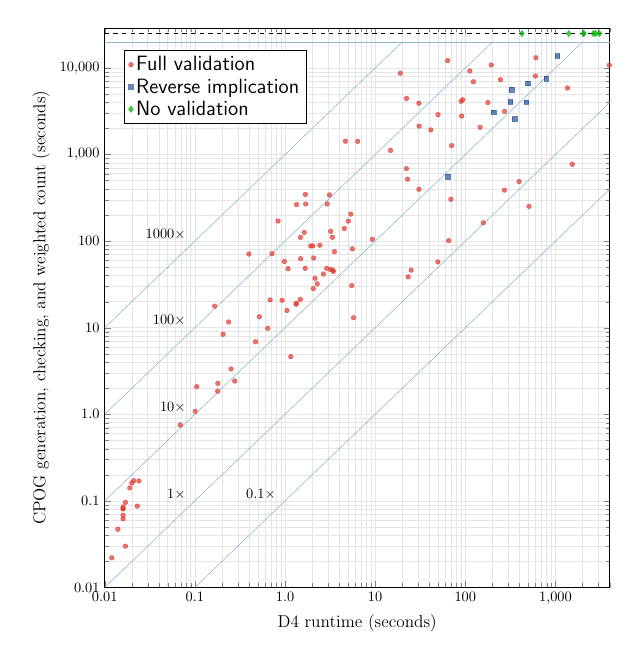
\begin{tikzpicture}[scale = 0.52]
  \begin{axis}[mark options={scale=0.55},grid=both, grid style={black!10}, ymode=log,
      legend style={at={(0.4,0.96)}},
      legend cell align={left},
                              x post scale=1.8, y post scale=2.4,
                              xmode=log,xmin=0.01,xmax=4000,
                              xtick={0.01, 0.1,1.0,10,100,1000,10000}, xticklabels={0.01, 0.1, 1.0, 10, 100, {1,000}, {10,000}},
                              ymin=0.01, ymax=29000,
                              ytick={0.01, 0.1,1.0,10,100,1000,10000,100000}, yticklabels={0.01, 0.1, 1.0, 10, 100, {1,000},{10,000},{100,000}},
                              xlabel={\large D4 runtime (seconds)}, ylabel={\large CPOG generation, checking, and weighted count  (seconds)},
%                              title={D4 Defining Clause Generation}
            ]
%    \input{data-formatted/time-d4-verify}
\addplot [only marks, color=redorange, mark=*,  mark options={scale=0.8}, opacity=0.7] coordinates { (5.758,13.045) (0.017,0.03) (0.014,0.047) (0.179,1.847) (0.016,0.062) (0.012,0.022) (0.024,0.16999999999999998) (0.928,20.743000000000002) (0.069,0.754) (0.166,17.75) (1.48,21.223999999999997) (3.356,110.95) (3.184,47.193) (1.676,48.49) (0.016,0.08099999999999999) (0.019,0.141) (0.472,6.882) (0.02,0.161) (5.048,170.314) (0.398,70.944) (0.685,20.974) (0.252,3.342) (30.753,2129.125) (0.643,9.855) (2.154,37.226) (1.158,4.633) (2.436,89.771) (1.636,126.078) (1.491,62.69) (4.683,1426.489) (30.566,3914.6259999999997) (145.967,2062.9629999999997) (2.666,41.732) (0.105,2.084) (5.508,30.682000000000002) (244.952,7312.937) (0.206,8.398) (606.378,13144.747) (23.234,38.677) (0.837,170.78900000000002) (49.574,57.587999999999994) (25.077,46.29900000000001) (63.691,12177.898) (4.544,139.899) (1.679,346.404) (22.322,4447.67) (2.076,63.914) (70.355,1268.879) (90.915,2782.6130000000003) (123.037,6933.090999999999) (112.248,9251.585) (178.14,3991.669) (394.71,487.715) (158.115,163.04700000000003) (69.122,304.792) (508.972,252.11700000000002) (2.033,88.145) (270.954,388.37300000000005) (1536.914,771.949) (19.013,8702.097) (2.938,269.092) (598.709,8085.308) (9.311,105.24799999999999) (0.277,2.423) (0.101,1.0819999999999999) (30.577,397.437) (0.18,2.276) (0.016,0.08499999999999999) (0.021,0.17099999999999999) (0.52,13.385) (0.016,0.081) (0.237,11.658000000000001) (0.985,58.235) (2.278,32.183) (1.053,15.828) (1.326,18.72) (2.908,48.425) (3.441,44.796) (2.06,28.279) (1.483,110.438) (3.377,46.214) (0.017,0.096) (0.016,0.068) (3.536,75.644) (1.337,19.128) (5.587,81.44800000000001) (193.799,10831.611) (89.858,4126.2029999999995) (0.023,0.087) (49.796,2888.948) (0.718,71.703) (5.364,205.144) (3.21,129.792) (41.455,1926.9289999999999) (1.083,48.012) (1.695,268.74) (1.345,264.555) (3.111,342.282) (6.397,1421.771) (22.214,688.805) (65.322,101.219) (22.917,519.913) (272.642,3145.4440000000004) (1.929,87.996) (1358.165,5874.534000000001) (3951.002,10775.298999999999) (14.808,1115.634) (93.537,4308.5650000000005)};

%    \input{data-formatted/time-d4-verify-onesided-only}
\addplot [only marks, color=bluegray, mark=square*,  mark options={scale=0.8}, opacity=0.7] coordinates { (205.743,3092.184) (326.575,5611.652) (476.021,4030.371) (494.38,6625.9839999999995) (1046.603,13782.805) (351.999,2582.8019999999997) (64.21,557.361) (316.505,4054.794) (788.377,7536.77)};

%    \input{data-formatted/time-d4-failure}
\addplot [only marks, color=darkgreen, mark=diamond*, mark options={scale=1.1}, opacity=0.7] coordinates { (2052.239,25000) (424.73,25000) (2636.562,25000) (1403.431,25000) (3070.214,25000) (2053.446,25000) (2790.169,25000)};

    \legend{
      \scriptsize \textsf{\Large Full validation},
      \scriptsize \textsf{\Large Reverse implication},
      \scriptsize \textsf{\Large No validation},
    }
    \addplot[mark=none, dashed] coordinates{(0.01,25000) (4000, 25000)};
    \addplot[mark=none, color=lightblue] coordinates{(0.01,20000) (4000,20000)};
    \addplot[mark=none, color=lightblue] coordinates{(0.1,0.01) (10000.0,1000.0)};
    \addplot[mark=none, color=lightblue] coordinates{(0.01,0.01) (10000.0,10000.0)};
    \addplot[mark=none, color=lightblue] coordinates{(0.01,0.1) (2000,20000)};
    \addplot[mark=none, color=lightblue] coordinates{(0.01,1.0) (200, 20000)};
    \addplot[mark=none, color=lightblue] coordinates{(0.01,10.0) (20, 20000)};
    \node[left] at (axis cs: 0.9,0.12) {$0{.}1\times$};
    \node[left] at (axis cs: 0.09,0.12) {$1\times$};
    \node[left] at (axis cs: 0.09,1.2) {$10\times$};
    \node[left] at (axis cs: 0.09,12.0) {$100\times$};
    \node[left] at (axis cs: 0.09,120.0) {$1000\times$};

          \end{axis}
\end{tikzpicture}
\end{center}
\end{minipage}
\begin{minipage}{0.28\textwidth}
{\bf Ratios}

\medskip

Min\\
\-\hspace{2ex} 0.5$\times$

\medskip

Harmonic mean\\
\-\hspace{2ex} 5.9$\times$

\medskip

Median\\
\-\hspace{2ex} 16.4$\times$


\medskip

Max\\
\-\hspace{2ex} 465.8$\times$
\end{minipage}
\end{frame}

\begin{frame}
\frametitle{Experimental Results: CPOG Sizes}
\bigskip
\begin{minipage}{0.73\textwidth}
\begin{center}
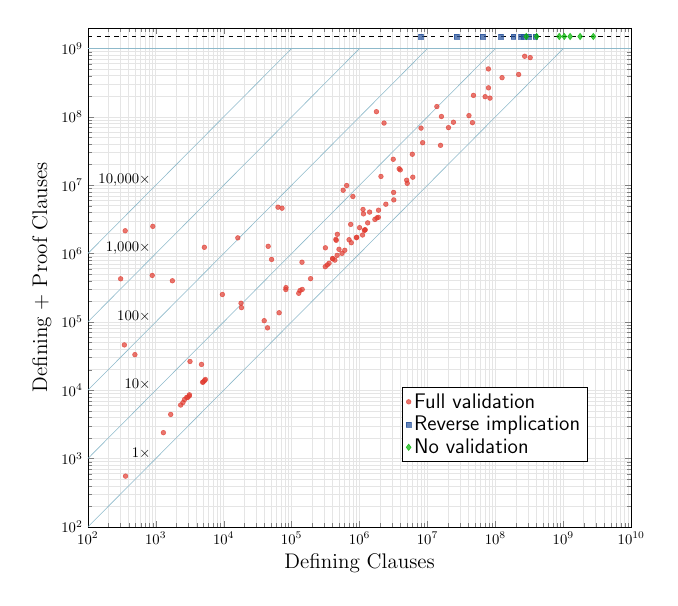
\begin{tikzpicture}[scale = 0.53]
  \begin{axis}[mark options={scale=0.55},grid=both, grid style={black!10},
      legend style={at={(0.92,0.28)}},
      legend cell align={left},
                              x post scale=1.9, y post scale=2.10,
                              xmode=log,xmin=100,xmax=1e10, 
                              xtick={100,1000, 10000, 100000, 1000000, 10000000, 100000000, 1000000000, 1e10}, 
                              xticklabels={$10^2$,$10^3$,$10^4$,$10^5$,$10^6$,$10^7$,$10^8$,$10^9$, $10^{10}$},
                              ymode=log, ymin=100, ymax=2000000000, 
                              ytick={100,1000, 10000, 100000, 1000000, 10000000, 100000000, 1000000000},
                              yticklabels={$10^2$,$10^3$,$10^4$,$10^5$,$10^6$,$10^7$,$10^8$,$10^9$},
                              xlabel={\Large Defining Clauses}, ylabel={\Large Defining + Proof Clauses},
            ]
%    \input{data-formatted/defining+total}
\addplot [only marks, color=redorange, mark=*,  mark options={scale=0.8}, opacity=0.7] coordinates { (18271,161794) (1295,2397) (1659,4427) (127284,262373) (2325,6077) (359,554) (5373,14373) (314359,1213826) (44178,81780) (493,33207) (605988,1117440) (1141369,3809317) (1197649,2211944) (1001050,2393131) (2947,7851) (4991,13207) (355617,721935) (4897,13101) (2437497,5273728) (345,46079) (701346,1593947) (3191,26378) (5985623,28392373) (467550,940819) (1318024,2813565) (4713,23892) (1682059,3160386) (1406192,4043887) (899701,1704811) (4936014,11840667) (8038928,68469623) (70651620,197339867) (9567,251890) (39501,104182) (18007,187551) (125319627,374762287) (82194,297768) (269645146,770382773) (304,427342) (574062,8448281) (887,478450) (1757,399856) (78873354,503117290) (190248,429409) (2064844,13434107) (13737124,141587875) (50722,820648) (45923418,82243431) (83111464,188103550) (40776253,104351646) (79106742,265990284) (3133905,23973053) (16147,1697847) (45214,1277037) (72258,4612352) (905,2500003) (401032,840020) (355,2155900) (63050,4771522) (3195277,6098685) (1125105,4417869) (325251378,736764776) (6074672,13104909) (132891,287958) (65522,136116) (15561156,38336288) (143191,298755) (2851,7851) (5243,13911) (334862,681444) (2659,7335) (82585,317789) (447979,1612224) (905899,1733678) (433226,802268) (551970,1006319) (1891045,3387533) (1210098,2232426) (755273,1440924) (470934,1914084) (1178453,2188886) (3131,8575) (2515,6607) (1903735,4312279) (1107098,1868005) (1801878,3324418) (47556240,206213289) (24087642,83491057) (3109,8227) (16038150,101261480) (312728,642675) (3175308,7847036) (142059,747752) (20382514,69650789) (453769,1563728) (498246,1154507) (797866,6840229) (3835114,17412807) (5035130,10668725) (647011,9905453) (5189,1234644) (740235,2672407) (219979530,417455256) (402460,844395) (2295530,81147729) (1772352,119113610) (3975194,16763326) (8493275,41873955)};

%    \input{data-formatted/clauses-defining-onesided}
%\addplot [only marks, color=bluegray, mark=square*, mark options={scale=0.8}, opacity=0.7] coordinates { (120863325,120863325) (184240761,184240761) (7992626,7992626) (260104055,260104055) (387150630,387150630) (65210486,65210486) (26816878,26816878) (238009358,238009358) (307380236,307380236)};
\addplot [only marks, color=bluegray, mark=square*, mark options={scale=0.8}, opacity=0.7] coordinates { (120863325,1500000000) (184240761,1500000000) (7992626,1500000000) (260104055,1500000000) (387150630,1500000000) (65210486,1500000000) (26816878,1500000000) (238009358,1500000000) (307380236,1500000000)};

%    \input{data-formatted/clauses-defining-failure}
\addplot [only marks, color=darkgreen, mark=diamond*, mark options={scale=1.1}, opacity=0.7] coordinates { (284769023,1500000000) (404276843,1500000000) (1765743261,1500000000) (869865958,1500000000) (2761457765,1500000000) (1258914451,1500000000) (1030698214,1500000000)};

    \legend{
      \scriptsize \textsf{\Large Full validation},
      \scriptsize \textsf{\Large Reverse implication},
      \scriptsize \textsf{\Large No validation},
    }
    \addplot[mark=none, color=lightblue] coordinates{(100,1e9) (1e10,1e9)};
    \addplot[mark=none, color=lightblue] coordinates{(100,100) (1e9,1e9)};
    \addplot[mark=none, color=lightblue] coordinates{(100,1000) (1e8,1e9)};
    \addplot[mark=none, color=lightblue] coordinates{(100,10000) (1e7,1e9)};
    \addplot[mark=none, color=lightblue] coordinates{(100,100000) (1e6,1e9)};
    \addplot[mark=none, color=lightblue] coordinates{(100,1000000) (1e5,1e9)};
    \addplot[color=black,dashed] coordinates{(1e2,1.5e9) (1e10,1.5e9)};
    \node[left] at (axis cs: 1000,1200) {$1\times$};
    \node[left] at (axis cs: 1000,12000) {$10\times$};
    \node[left] at (axis cs: 1000,120000) {$100\times$};
    \node[left] at (axis cs: 1000,1200000) {$1{,}000\times$};
    \node[left] at (axis cs: 1000,12000000) {$10{,}000\times$};

          \end{axis}
\end{tikzpicture}
\end{center}
\end{minipage}
\begin{minipage}{0.25\textwidth}
{\bf Ratios}

\medskip

Min\\
\-\hspace{2ex} 1.5$\times$

\medskip

Harmonic mean\\
\-\hspace{2ex} 3.1$\times$

\medskip

Median\\
\-\hspace{2ex} 2.7$\times$

\medskip

Max\\
\-\hspace{2ex} 6073.0$\times$
\end{minipage}
\end{frame}


\begin{frame}
  \frametitle{Final Thoughts}

  \medskip

  {\bf Observations}
  \begin{itemize}
  \item Toolchain can handle all but largest outputs from D4
  \item Framework is very general
    \begin{itemize}
      \bitem E.g., can generate, prove, and apply lemmas without any extensions
      \bitem Not tied to particular compilation method
    \end{itemize}
  \end{itemize}

  \medskip

  {\bf Future Work}
  \begin{itemize}
  \item Improve speed and capacity of toolchain
  \item Handle outputs from other knowledge compilers
  \item Certification of other automated reasoning tools
  \end{itemize}

\end{frame}

\begin{frame}
\frametitle{Supplementary Information}

\medskip
{\bf Code}
\begin{center}
 \hcref{https://github.com/rebryant/cpog}
\end{center}
{\bf Documentation}
\begin{center}
 \hcref{https://doi.org/10.5281/zenodo.7966174}
\end{center}
\begin{itemize}
\item Worked example
\item More details on algorithms
\item More details on formal verification
\item Lots of experimental results
\end{itemize}

\end{frame}


\begin{frame}

  \frametitle{References}

\medskip

\begin{minipage}{0.1\textwidth}
    \textcolor{white}{Filler}
\end{minipage}
\begin{minipage}{0.88\textwidth}
\footnotesize
\begin{itemize}

\item[CapLagMar-2021]
  F. Capelli, J.-M. Lagniez, and P. Marquis,
  ``Certifying top-down decision-{DNNF} compilers'',
  \structure{AAAI}, 2021

\item[DarMar-2002]
  A. Darwiche and P. Marquis,
  ``A knowledge compilation map,''
  \structure{JAIR}, 2002
  
\item[DemUlr-2021]
  L. de Moura and S. Ulrich,
  ``The Lean 4 theorem prover and programming language,''
\structure{CADE},  2021

\item[FicHecRol-2022]
  J. Fichte, M. Hecher, and V. Roland,
  ``Proofs for propositional model counting,''
  \structure{SAT} 2022.

\item[HeuHunWet-2013] M. J. H. Heule, W. A. Hunt, Jr., N. Wetzler,
  ``Trimming while checking clausal proofs,''
  \structure{FMCAD}, 2013.


%%\item[KimVdbDra-2017] Angelika Kimmig, Guy Van den Broeck, and Luc De Raedt,
%%  ``Algebraic model counting,''
%%  \structure{J. Applied Logic}, 2017

\item[LagMar-2017] J.-M. Lagniez and  P. Marquis,
  ``An improved decision-DNNF compiler,''
  \structure{IJCAI}, 2017
\end{itemize}
\end{minipage}
\end{frame}

\end{document}

\begin{frame}
  \frametitle{Old Slides}
\end{frame}

\begin{frame}

   \frametitle{Algebraic Formulation}
   \begin{itemize}
     \item Inspired by Kimmig et al. \reference{KimVdbDra-2017}
   \end{itemize}

\medskip
{\bf Ring Evaluation}
\begin{itemize}
     \item Commutative ring ${\cal R}$ 
     \item Assign weight $w(x_i) \in {\cal R}$ to each input variable $x_i$
     \item Define $w(\xnot_i) = 1-w(x_i)$
       \begin{itemize}
         \bitem Write as $\pneg w(x_i)$
       \end{itemize}
     \item Ring evaluation ${\bf R}(\phi, w)$ of formula $\phi$:
   \end{itemize}
   \begin{eqnarray*}
     {\bf R}(\phi, w) & = & \sum_{\alpha \in {\cal M}(\phi)} \; \prod_{\ell_i \in \alpha} w(\ell_i)
   \end{eqnarray*}
\end{frame}

\begin{frame}
\frametitle{Ring Evaluation Examples}

\bigskip

{\bf Model Counting}
\begin{itemize}
\item Let $w(x_i) = w(\oneg{x}_i) = 1/2$ for all $i$
\item ${\bf R}(\phi, w)$ gives \structure{density} of function
  \begin{itemize}
    \bitem Fraction of assignments that satisfy $\phi$
  \end{itemize}
\item Scale by $2^n$ to get model count
\end{itemize}

\medskip

{\bf Probabilistic Inference}
\begin{itemize}
\item Each input variable $x_i$ is true with probability $p(x_i)$
\item ${\bf R}(\phi, p)$ is probability that formula is true
\end{itemize}

\medskip

{\bf Weighted Model Counting}
\begin{itemize}
\item Literals can have weights $W$ such that $W(x_i) + W(\oneg{x}_i) \not = 1$
\item Handle by normalizing and scaling  
\end{itemize}

\end{frame}

\begin{frame}
\frametitle{Forward Proof Generation: Monolithic Method}
\vskip -1.0em
\begin{eqnarray*}
             \phi_I(X) & \Longrightarrow & \exists!\,Z\; \theta_P(X, Z)
\end{eqnarray*}
%\vskip -0.5em

           {\bf Method:}

           \medskip
           
           \begin{itemize}
             \item Use SAT solver to generate proof that $\phi_I \land \neg \theta_P$ unsatisfiable
             \item Negate $\theta_P$ by replacing unit clause $[r]$ with $[\oneg{r}]$
           \end{itemize}

           \bigskip

           {\bf Properties:}
           
           \medskip

           \begin{itemize}
           \item No assumption about how POG was generated
             \begin{itemize}
               \bitem Works when run preprocessor before D4
             \end{itemize}
             \item Experimentally: Scales to POGs with  $\sim 10^6$ defining clauses
           \end{itemize}


\end{frame}

\begin{frame}
\frametitle{Forward Proof Generation: Structural Method}
\vskip -1.0em
\begin{eqnarray*}
             \phi_I(X) & \Longrightarrow & \exists!\,Z\; \theta_P(X, Z)
\end{eqnarray*}
%\vskip -0.5em

           {\bf Method:}

           \medskip

           \begin{itemize}
           \item Generate proof by recursive traversal of POG
           \item Call SAT solver for some subformulas
           \item Avoid exponential expansion using lemmas
             \begin{itemize}
               \bitem Prove lemma when encounter node with indegree $\geq 2$
               \bitem Apply lemma and stop recursion when encounter again
               \bitem Can express lemmas within CPOG framework
             \end{itemize}
           \end{itemize}

          {\bf Properties:}

          \begin{itemize}
           \item Assumes POG generated by top-down knowledge compiler
           \item Experimentally: Scales to POGs with $\sim 10^8$ defining clauses
          \end{itemize}

\end{frame}



\begin{frame}
\frametitle{CPOG Declaration + Proof}
           \medskip

           {\bf Input Formula $\phi_I$}

           \medskip
           
           {\bf POG Declaration $\theta_P$}
           \begin{itemize}
             \item Tseitin encoding of POG
             \item Extension variable $u$ for each operation node  $\nodeu$
             \item Node $\nodeu$ with $k$ children characterized  by $k+1$ defining clauses
             \item Each child indicated by literal
               \begin{itemize}
                 \bitem Positive or negated argument
                 \bitem Input variable or result from other operation
               \end{itemize}
             \item Unit clause $[r]$ for root node $\noder$
           \end{itemize}

           \bigskip

           {\bf Proof Objective}
\vskip -1.0em
           \begin{eqnarray*}

           \end{eqnarray*}
\vskip -0.5em
         \begin{itemize}
         \item Transform $\phi_I$ into $\theta_P$ via equivalence-preserving proof steps
         \end{itemize}

\end{frame}



\begin{frame}
  \frametitle{CPOG Format: Operations}

\begin{center}
\only<1>{
%% Hold space for table.  This should be invisible
\textcolor{white}{
  \begin{tabular}{lllll}
    \toprule
    \multicolumn{4}{c}{Rule} & \multicolumn{1}{l}{Description} \\
    \midrule
    \makebox[5mm][l]{\wtext{$C$}} & \makebox[10mm][l]{\texttt{p}}  & \makebox[15mm][l]{$\wtext{V} \; \wtext{L^{*}}$ \texttt{0}} & \makebox[15mm][l]{}  & \makebox[20mm][l]{Declare $\pand$ operation} \\
    \wtext{$C$}    & \texttt{s} & $\wtext{V} \; \wtext{L \; L}$    & \wtext{$C^{+}$} \texttt{0}  & Declare $\por$ operation \\
    \bottomrule
  \end{tabular}
}} %% End of placeholder
\only<2->{
  \begin{tabular}{lllll}
    \toprule
    \multicolumn{4}{c}{Rule} & \multicolumn{1}{l}{Description} \\
    \midrule
    \makebox[5mm][l]{\rtext{$C$}} & \makebox[10mm][l]{\texttt{p}}  & \makebox[15mm][l]{$\btext{V} \; \gtext{L^{*}}$ \texttt{0}} & \makebox[15mm][l]{}  & \makebox[20mm][l]{Declare $\pand$ operation} \\
    \rtext{$C$}    & \texttt{s} & $\btext{V} \; \gtext{L \; L}$    & \rtext{$C^{+}$} \texttt{0}  & Declare $\por$ operation \\
    \bottomrule
  \end{tabular}
}
  \medskip

    \begin{tabular}{llllll}
      \makebox[2mm][l]{\rtext{$C$}} & \makebox[18mm][l]{Clause ID} & 
      \makebox[2mm][l]{\btext{$V$}} & \makebox[15mm][l]{Variable} &
      \makebox[2mm][l]{\gtext{$L$}} & \makebox[15mm][l]{Literal} \\
    \end{tabular}
\end{center}

  \medskip

  \begin{minipage}{0.4\textwidth}
  \centering{
  \input{dd/eg4-partial}
  }
  \end{minipage}
  \begin{minipage}{0.58\textwidth}
  \centering{
    \begin{tabular}{lll}
    \toprule
    \makebox[5mm]{ID} & \multicolumn{2}{l}{CPOG line}  \\
    \midrule
    \rtext{6} & \texttt{p \btext{5} \gtext{-3 -4}} & \texttt{0} \\
    \rtext{9} & \texttt{p \btext{6} \gtext{3 4}} & \texttt{0} \\
    \rtext{12} & \texttt{s \btext{7} \gtext{5 6} \rtext{7 10}} & \texttt{0} \\
    \bottomrule
    \end{tabular}
  }
  \end{minipage}

  \medskip

\only<2->{
  \begin{itemize}
    \item Operation with $k$ arguments generates $k+1$ defining clauses
      \begin{itemize}
        \bitem Operation with ID $i$ generates clauses $i$ through $i+k$
      \end{itemize}
    \item $\por$ operation includes clause IDs for mutual exclusion proof
  \end{itemize}
}
\end{frame}


\begin{frame}
  \frametitle{CPOG Format: Clause addition and deletion}

\bigskip

\begin{center}
  \begin{tabular}{lllll}
    \toprule
    \multicolumn{4}{c}{Rule} & \multicolumn{1}{l}{Description} \\
    \midrule
    \makebox[5mm][l]{\rtext{$C$}} & \makebox[10mm][l]{\texttt{a}}  & \makebox[15mm][l]{$\gtext{L^{*}}$ \texttt{0}} & \makebox[15mm][l]{$\rtext{C^{+}}$ \texttt{0}}  & \makebox[20mm][l]{Add RUP clause} \\
     & \texttt{d} & \rtext{$C$}             & \rtext{$C^{+}$}  \texttt{0} & Delete RUP clause \\
    \bottomrule
  \end{tabular}
\end{center}

\bigskip

\begin{itemize}
\item $\gtext{L^{*}}$ declares literals in clause
\item $\rtext{C^{+}}$ provides hint for reverse unit propagation (RUP) proof
\item Can only add clause if it is implied by existing ones
\item Can only delete clause if it is implied by remaining ones
\end{itemize}

\end{frame}



\begin{frame}
  \frametitle{CPOG Format: Root Literal}

\bigskip

\begin{center}
  \begin{tabular}{lllll}
    \toprule
    \multicolumn{4}{c}{Rule} & \multicolumn{1}{l}{Description} \\
    \midrule
     \makebox[5mm][l]{} & \makebox[10mm][l]{\texttt{r}} & \makebox[15mm][l]{\gtext{$L$}}    & \makebox[7mm][l]{}            & \makebox[28mm][l]{Declare root literal}\\
    \bottomrule
  \end{tabular}
\end{center}

\bigskip

\begin{itemize}
\item Declare POG root
\end{itemize}

\bigskip

{\bf Observations about CPOG format:}

\medskip

\begin{itemize}
\item Builds on standard clausal proof formats
\item Not based on any particular compilation method
\end{itemize}  

\end{frame}



\begin{frame}

  \frametitle{Proof Goal: Tseitin Equivalence}


  \begin{itemize}
  \item Formula $\psi(X, Z)$
  \item Tseitin variables $Z$
   \end{itemize}

\medskip

{\bf Tseitin Satisfiability}

\smallskip

For any assignment $\alpha$ to variables in $X$, either:
  \begin{enumerate}
    \item There is a unique assignment $\alpha^Z$ to the variables in $X \cup Z$ such that $\alpha^Z$ satisfies $\psi$, or
    \item There is no assignment $\alpha^Z$ to the variables in $X \cup Z$ such that $\alpha^Z$ satisfies $\psi$
   \end{enumerate}

\medskip

{\bf Tseitin Equivalence}
\vskip -1ex
\begin{eqnarray*}
  \psi_1(X, Z_1) & \tequiv & \psi_2(X, Z_2)
\end{eqnarray*}
\vskip -1ex
\begin{itemize} 
\item For any assignment $\alpha$ to the variables in $X$, either both $\psi_1$ and $\psi_2$ are Tseitin satisfiable, or neither are.
\end{itemize}

\end{frame}

\begin{frame}
\frametitle{CPOG Proof Objective}

           \begin{eqnarray*}
             \phi_I(X, \emptyset) & \tequiv & \theta_P(X, Z)
           \end{eqnarray*}

\begin{itemize}
\item $Z$: extension variables representing the POG operations
\item Assignment $\alpha$ to $X$ satisfies $\phi_I$ if and only if there is a unique assignment to the POG variables such that $\theta_P$ is also satisfied
  \begin{itemize}
    \bitem Defining clauses for POG
    \bitem Unit clause $[r]$
  \end{itemize}
\end{itemize}

\bigskip

{\bf Proof Methodology}
\begin{itemize}
\item Transform $\phi_I$ to $\theta_P$ by sequence of equivalence preserving proof steps
\end{itemize}


\end{frame}



